\chapter{实验设计与结果分析}\label{chap:experiments}

本章给出论文主要实验。实验不只看单次最优值，而是围绕四个可检查的问题展开：复杂区域内能否得到非支配部署方案；在同一评价预算下，MOPSO-DT改进配置与经典多目标算法相比处在什么位置；坐标变换对边界任务点是否有帮助；ECR与$J_{\min}$之间的取舍在两个场景中是否稳定出现。
\section{实验设置与评价指标}

实验覆盖三类场景：Paper-Aligned场景用于验证雷达方程模型下的部署效果，Challenging场景用于多算法公平对比和困难传播条件测试，Tuning场景用于参数调优。表~\ref{tab:scenarios}给出场景配置，表~\ref{tab:mopso_params}给出MOPSO-DT主要参数。

三类场景的用途不同。Paper-Aligned场景保留雷达方程中的距离、增益和波长等物理量，用来检查算法在较完整物理参数下的部署结果；Challenging场景采用更快的指数衰减，便于拉开不同优化器和边界处理方式的差异；Tuning场景只用于内部参数选择，不参与主结论。这样划分后，调参、算法比较和结果解释不会混在同一组样本中。

\begin{table}[!htbp]
\centering
\small
\caption{实验场景配置}
\label{tab:scenarios}
\begin{tabular}{lccc}
\toprule
场景 & 区域规模 & 雷达数 & 传播模型 \\
\midrule
Paper-Aligned & 300km$\times$300km & 8 & 雷达方程 \\
Challenging & 200km$\times$200km & 8 & 指数衰减（$\beta=0.03$） \\
Tuning & $\sim$200km$\times$200km & 8 & 指数衰减（$\beta=0.01$） \\
\bottomrule
\end{tabular}
\end{table}
\begin{table}[!htbp]
\centering
\small
\caption{MOPSO-DT参数配置}
\label{tab:mopso_params}
\begin{tabular}{lcc}
\toprule
参数 & 原始配置 & 推荐配置 \\
\midrule
粒子数 $N_P$ & 20--50 & 50 \\
最大迭代 $T_{\max}$ & 30--50 & 100--500 \\
惯性权重策略 & legacy & standard \\
认知因子 $c_1$ & 2.0 & 2.0 \\
社会因子 $c_2$ & 2.0 & 2.0 \\
基础变异率 $p_m^{\text{base}}$ & 0.0 & 0.01 \\
全局最优选择 & random & crowding \\
档案容量 & 100 & 100 \\
\bottomrule
\end{tabular}
\end{table}

评价指标包括有效覆盖率ECR、最小等效干扰强度$J_{\min}$、超体积HV、Spacing、ECR-$J_{\min}$相关系数和运行时间。其中，ECR和$J_{\min}$直接对应本文的覆盖与压制两个任务目标；HV用于综合评估非支配解集的收敛性和多样性~\cite{Zitzler2001}；Spacing用于衡量前沿分布均匀性，与拥挤距离等多样性维护机制具有相同的评价动机~\cite{Deb2002,Raquel2005}；ECR-$J_{\min}$相关系数用于描述同一Pareto档案内两个物理目标之间的经验性权衡，不作为严格统计显著性检验；运行时间则反映工程部署中的计算代价。新增的算法对比实验和边界专项实验均输出结构化JSON结果文件，并由绘图脚本自动生成论文图表。算法对比采用Challenging场景，所有方法使用相同任务点、相同目标函数、相同混合变量编码和相同评价预算，随机种子为2026、2027、2028。

\section{多算法对比实验}

为避免只与同源MOPSO变体比较导致结论过窄，本文在相同部署模型上引入五类基线算法：原始MOPSO-DT配置、NSGA-II-DT、MOEA/D-DT、SPEA2-DT和随机搜索。NSGA-II、MOEA/D和SPEA2分别代表非支配排序、分解式多目标优化和强度Pareto适应度三类经典算法思想~\cite{Deb2002,Zhang2007,Zitzler2001}；原始MOPSO-DT配置用于衡量本文参数和领导者选择调整的边际贡献；随机搜索用于提供不依赖群体进化机制的下界参考。算法名称中的``-DT''表示其均复用本文的区域分解、坐标变换和统一评估函数，差异仅在种群更新和选择机制。

表~\ref{tab:algorithm_comparison}给出了Challenging场景下六种方法的三种子统计结果。图~\ref{fig:algorithm_pareto_overlay}展示各方法在ECR-$J_{\min}$空间中的非支配解分布，图~\ref{fig:algorithm_metrics_bars}和图~\ref{fig:runtime_quality_tradeoff}进一步展示HV、Spacing、解数量和运行时间之间的关系。

\begin{table}[!htbp]
\centering
\small
\caption{Challenging场景下同评价预算算法对比}
\label{tab:algorithm_comparison}
\begin{tabular}{lcccc}
\toprule
方法 & HV$\uparrow$ & Spacing$\downarrow$ & 解数 & 时间(s) \\
\midrule
本文MOPSO-DT & 0.0308$\pm$0.0015 & 0.0071$\pm$0.0029 & 14.0 & 58.3 \\
MOPSO-DT legacy & 0.0316$\pm$0.0017 & 0.0072$\pm$0.0033 & 13.7 & 61.5 \\
NSGA-II-DT & 0.0340$\pm$0.0002 & 0.0030$\pm$0.0008 & 70.3 & 61.5 \\
MOEA/D-DT & 0.0348$\pm$0.0002 & 0.0037$\pm$0.0012 & 59.0 & 62.6 \\
SPEA2-DT & 0.0340$\pm$0.0002 & 0.0017$\pm$0.0002 & 86.7 & 71.6 \\
随机搜索 & 0.0322$\pm$0.0006 & 0.0031$\pm$0.0006 & 15.3 & 59.3 \\
\bottomrule
\end{tabular}
\end{table}

\begin{figure}[!htbp]
\centering
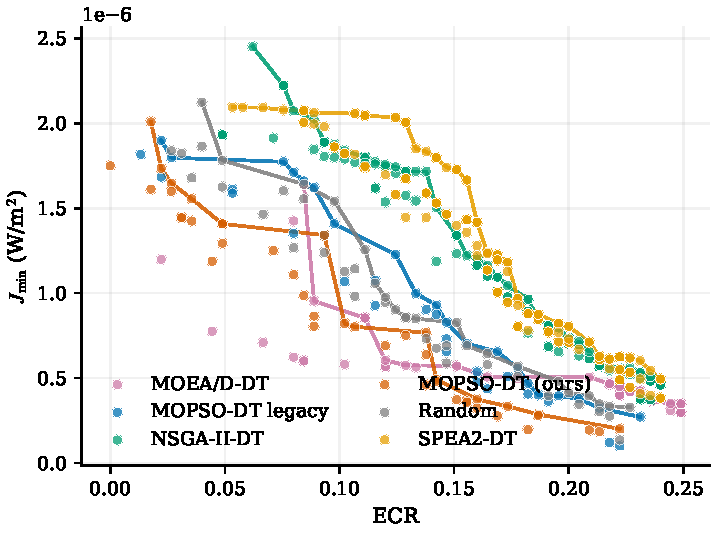
\includegraphics[width=0.86\linewidth]{figures/algorithm_pareto_overlay.pdf}
\caption{不同算法的ECR-$J_{\min}$非支配解分布。}
\label{fig:algorithm_pareto_overlay}
\end{figure}

\begin{figure}[!htbp]
\centering
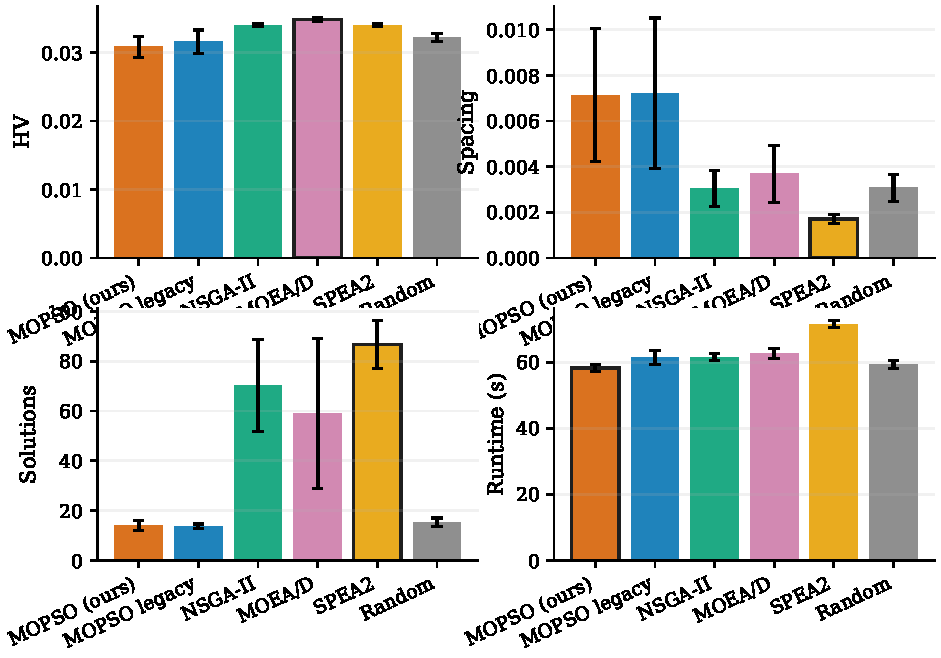
\includegraphics[width=0.88\linewidth]{figures/algorithm_metrics_bars.pdf}
\caption{不同算法的质量指标与运行时间对比。}
\label{fig:algorithm_metrics_bars}
\end{figure}

\begin{figure}[!htbp]
\centering
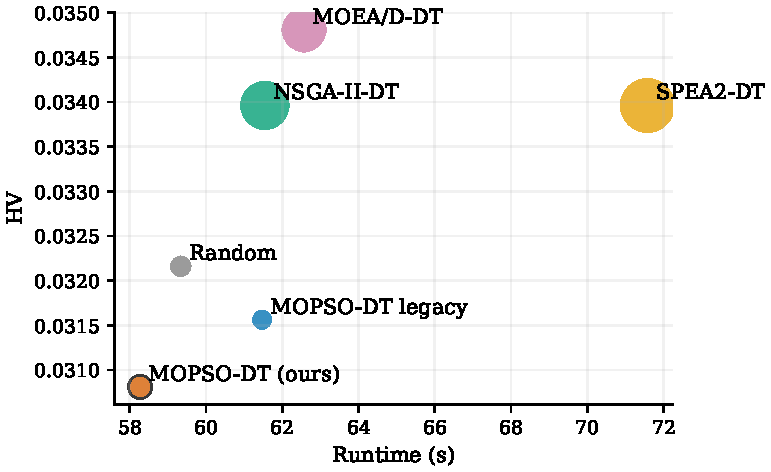
\includegraphics[width=0.80\linewidth]{figures/runtime_quality_tradeoff.pdf}
\caption{运行时间与HV的质量-效率权衡。}
\label{fig:runtime_quality_tradeoff}
\end{figure}

表中结果比较清楚：在Challenging场景下，MOEA/D-DT的平均HV最高，SPEA2-DT的Spacing最低，NSGA-II-DT保留的非支配解数量也更多。因此，本章不把本文MOPSO-DT配置写成“全面优于”经典MOEA方法。它的优势更多体现在与区域分解、坐标变换和异构传播评估的结合，以及相对legacy配置的可复现实验改进。

从图~\ref{fig:algorithm_pareto_overlay}可以看到，经典MOEA方法在固定预算下更容易铺开较密的前沿。MOPSO-DT类方法给出的解数较少，但粒子编码中显式包含子区域选择，所有候选解都会经过同一坐标映射再评估。本文改进配置相对legacy配置的收益不主要来自某一次HV绝对值，而来自更稳定的前沿分布、可复现的参数组合，以及后续边界实验中更清楚的几何约束解释。

\begin{figure}[!htbp]
\centering
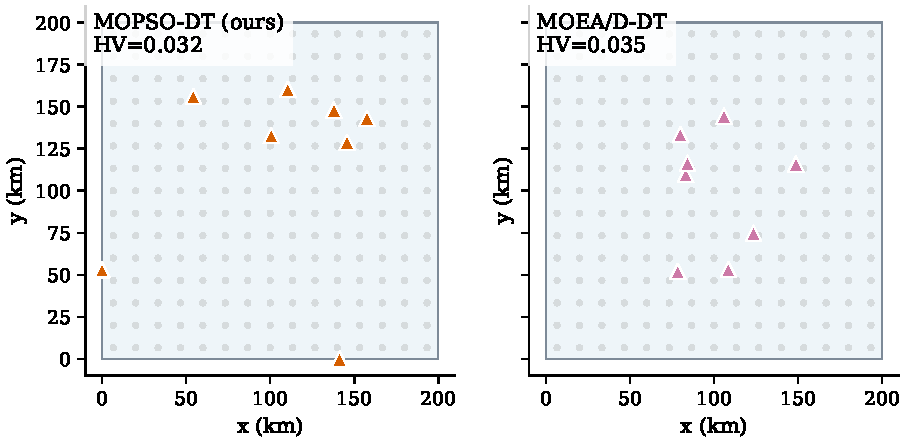
\includegraphics[width=0.90\linewidth]{figures/knee_deployment_comparison.pdf}
\caption{拐点部署方案对比。}
\label{fig:knee_deployment_comparison}
\end{figure}

\section{边界效应验证}

边界实验单独使用L形区域，是为了避免总体ECR把边缘问题掩盖掉。实验沿内外边界附近布置任务点，并比较坐标变换、直接物理空间搜索、legacy配置和NSGA-II-DT。各方法使用相同粒子规模、迭代次数和随机种子。表~\ref{tab:boundary_analysis}记录每个方法在档案中边界ECR最高解的平均结果，图~\ref{fig:boundary_coverage_map}展示其中一组覆盖图。

\begin{table}[!htbp]
\centering
\small
\caption{L形区域边界ECR专项实验}
\label{tab:boundary_analysis}
\begin{tabular}{lcccc}
\toprule
方法 & Overall ECR & Boundary ECR & Gap & HV \\
\midrule
本文坐标变换 & 0.319 & 0.156 & 0.163 & 0.0448 \\
直接物理空间 & 0.271 & 0.156 & 0.115 & 0.0412 \\
MOPSO-DT legacy & 0.282 & 0.115 & 0.168 & 0.0452 \\
NSGA-II-DT & 0.347 & 0.076 & 0.271 & 0.0467 \\
\bottomrule
\end{tabular}
\end{table}

\begin{figure}[!htbp]
\centering
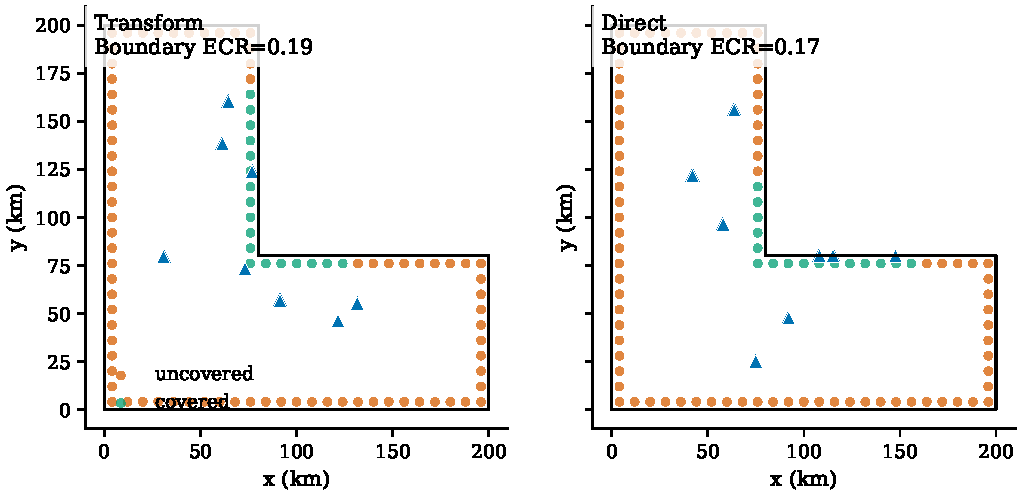
\includegraphics[width=0.90\linewidth]{figures/boundary_coverage_map.pdf}
\caption{边界任务点覆盖可视化。}
\label{fig:boundary_coverage_map}
\end{figure}

表~\ref{tab:boundary_analysis}的结果需要分开读。直接物理空间搜索的Boundary ECR最高，但整体ECR和HV较低；NSGA-II-DT在整体ECR和HV上占优，边界ECR却偏低。坐标变换方法位于二者之间，相对legacy配置和NSGA-II-DT改善了边界覆盖，但没有在所有边界指标上第一。因此，本文只把结论限定为缓解边界欠采样、改善部分边界覆盖表现。

这种现象也说明，边界ECR和整体ECR不是同一个目标。直接物理空间搜索可能把个别节点推到边界附近，从而覆盖更多边界点，但整体前沿不一定稳定。坐标变换方法的好处在于归一化候选点都能映射到合法区域，减少非法点剔除；代价是每次评估前多了一步几何映射，运行时间不会最低。

\section{参数调优与消融分析}

参数调优只在Tuning场景中完成，结果见表~\ref{tab:tuning_summary}。后续主实验沿用standard惯性权重、crowding领导选择和$p_m=0.01$作为改进配置，但调参结果显示该组合不是所有指标上的唯一最优。这里的调参结论只用于说明MOPSO-DT内部参数敏感性，不用于证明它优于所有外部算法。

\begin{table}[!htbp]
\centering
\small
\caption{参数调优结果汇总}
\label{tab:tuning_summary}
\begin{tabular}{lcccc}
\toprule
参数组合 & HV & Spacing & ECR范围 & $J_{\min}$范围 \\
\midrule
legacy + random + $p_m$=0 & 0.0310 & 0.0114 & [0.322, 0.560] & [0.039, 0.073] \\
legacy + crowding + $p_m$=0 & 0.0524 & 0.0145 & [0.131, 0.573] & [0.041, 0.083] \\
standard + random + $p_m$=0 & 0.0348 & 0.0091 & [0.198, 0.547] & [0.042, 0.070] \\
standard + random + $p_m$=0.01 & 0.0309 & 0.0315 & [0.247, 0.551] & [0.041, 0.068] \\
standard + crowding + $p_m$=0.01 & 0.0450 & 0.0175 & [0.176, 0.573] & [0.040, 0.080] \\
\bottomrule
\end{tabular}
\end{table}

\begin{table}[!htbp]
\centering
\small
\caption{惯性权重策略对比}
\label{tab:inertia_comparison}
\begin{tabular}{lccc}
\toprule
策略 & HV & Spacing & ECR范围 \\
\midrule
legacy & 0.0310 & 0.0114 & [0.322, 0.560] \\
standard & 0.0397 & 0.0202 & [0.229, 0.547] \\
adaptive & 0.0383 & 0.0138 & [0.204, 0.553] \\
\bottomrule
\end{tabular}
\end{table}

表~\ref{tab:inertia_comparison}显示，standard策略在该轮调参中取得更高HV，但Spacing并非最低；adaptive策略介于二者之间。crowding选择相对random能让粒子更多访问稀疏前沿区域，这与拥挤距离的设计目的一致~\cite{Deb2002,Raquel2005}。变异率方面，$p_m=0.01$提供少量区域编码扰动，但其效果依赖场景尺度和随机种子，因此本文不把单次调参结果写成绝对最优配置。

传播模型消融将空地异构传播模型替换为统一路径损耗模型，其余参数保持不变，结果见表~\ref{tab:ablation_prop}。

\begin{table}[!htbp]
\centering
\small
\caption{传播模型消融结果对比}
\label{tab:ablation_prop}
\begin{tabular}{lccc}
\toprule
配置 & Pareto解数 & ECR范围 & $r$ \\
\midrule
异构模型 & 11 & [0.036, 0.213] & --0.993 \\
统一模型 & 12 & [0.022, 0.218] & --0.972 \\
\bottomrule
\end{tabular}
\end{table}

统一传播模型得到的Pareto解数量和ECR范围与异构模型接近，但ECR-$J_{\min}$相关性发生变化。这个结果说明，异构传播模型的作用不是简单把某个指标抬高，而是改变空中节点和地面节点对覆盖、压制目标的贡献分配。对空地协同问题而言，这一点比单项数值提升更重要，因为统一模型会把A2G和G2G链路错误地视为同质链路。

坐标变换消融将垂直交点坐标变换替换为直接物理空间优化，测试边界可达性变化，结果见表~\ref{tab:ablation_transform}。

\begin{table}[!htbp]
\centering
\small
\caption{坐标变换消融结果对比}
\label{tab:ablation_transform}
\begin{tabular}{lccc}
\toprule
配置 & Pareto解数 & ECR范围 & 耗时(s) \\
\midrule
有坐标变换 & 15 & [0.000, 0.200] & 56.0 \\
无坐标变换 & 13 & [0.022, 0.204] & 18.5 \\
\bottomrule
\end{tabular}
\end{table}

有坐标变换时，档案中出现覆盖率很低的极端解，说明搜索确实到达了更偏边界或更不均衡的可行区域。无变换搜索更快，但可行域探索范围较窄。由此可见，坐标变换并不是为了缩短时间，而是为了在复杂区域中保留边界可达性。若区域接近规则矩形，可以采用直接搜索；若区域有凹边界、空洞或禁入区，坐标变换更有价值。

目标函数消融紧邻给出归一化目标函数与原始目标函数的对比，避免结果表与解释文字分离。

\begin{table}[!htbp]
\centering
\small
\caption{目标函数消融结果对比}
\label{tab:ablation_norm}
\begin{tabular}{lccc}
\toprule
配置 & Pareto解数 & ECR范围 & $r$ \\
\midrule
归一化 $f_2$ & 14 & [0.013, 0.209] & --0.931 \\
原始 $1/J_{\min}$ & 19 & [0.009, 0.191] & --0.982 \\
\bottomrule
\end{tabular}
\end{table}

目标函数消融显示，原始$1/J_{\min}$目标函数在Challenging场景下产生了更多Pareto解，且相关性绝对值更高。这是因为该场景ECR值本身较小，两个目标的量纲差异不如预期严重，$J_{\text{ref}}$的引入反而压缩了目标空间。归一化目标的价值更适合在量纲差异更大的场景中体现，例如雷达方程模型下ECR处于较高区间时，原始$1/J_{\min}$更容易在数值上主导搜索。该结果提示，目标函数归一化不应被机械视为总是更优，而应结合场景尺度和目标量纲进行选择。

\section{结果讨论}

本节回到本文方法本身，观察它在两个代表场景中给出的部署方案。表~\ref{tab:paper_aligned_summary}和表~\ref{tab:challenging_summary}列出结果范围，图~\ref{fig:paper_aligned_results}、图~\ref{fig:paper_aligned_pareto}和图~\ref{fig:challenging_scene}展示空间部署和目标空间分布。这里不再重复算法排名，而是看每组非支配解如何对应覆盖与压制之间的任务选择。

\begin{figure}[!htbp]
\centering
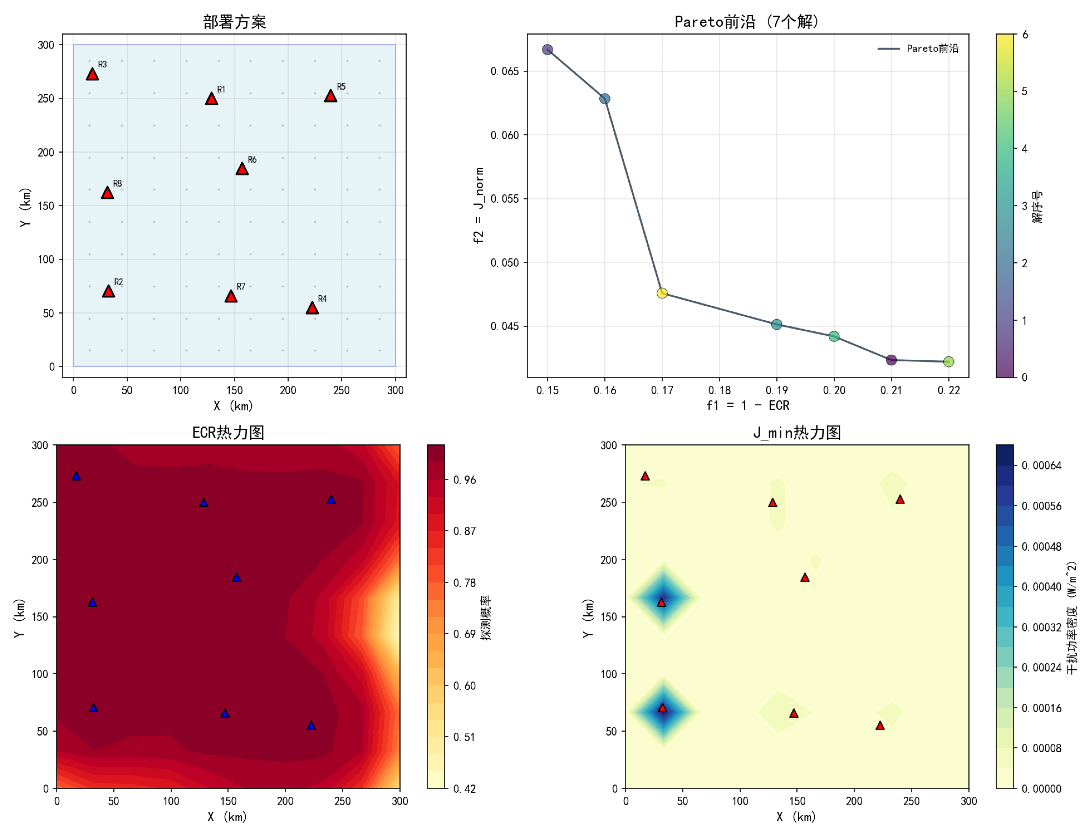
\includegraphics[width=0.88\linewidth]{figures/paper_aligned_results.pdf}
\caption{Paper-Aligned场景综合结果。}
\label{fig:paper_aligned_results}
\end{figure}

\begin{figure}[!htbp]
\centering
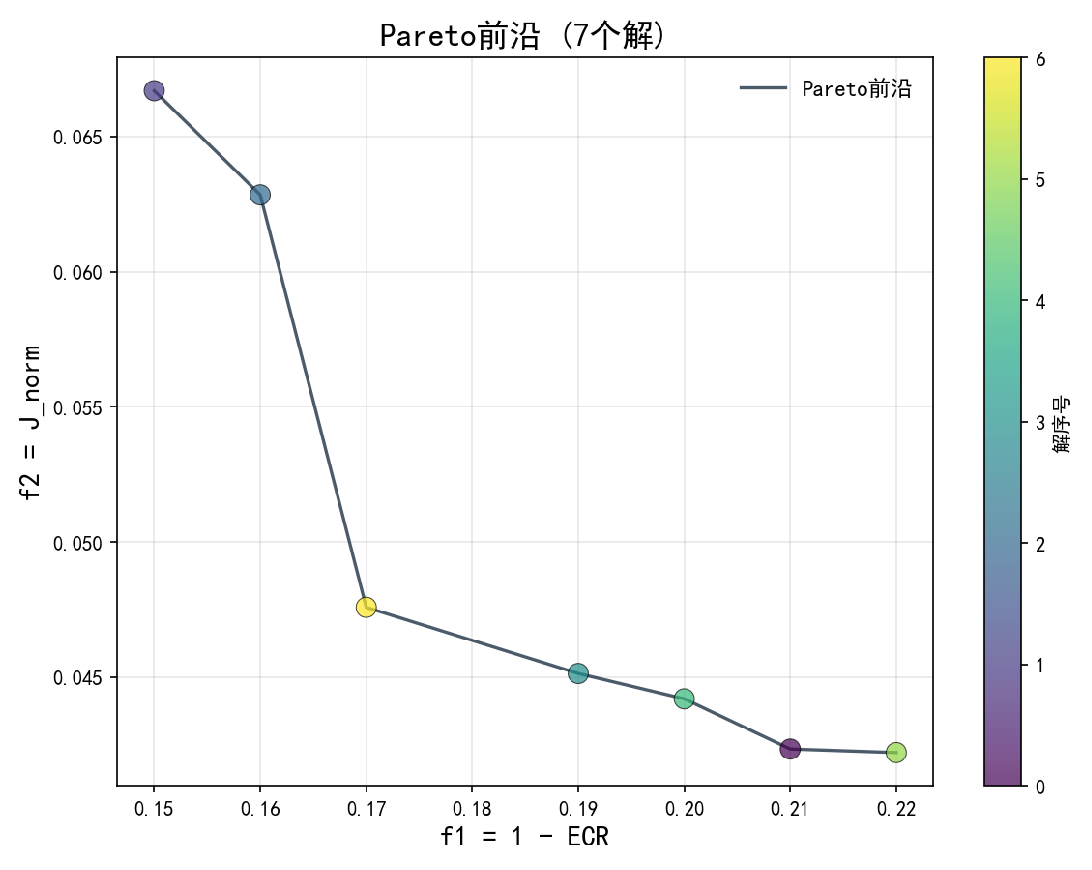
\includegraphics[width=0.88\linewidth]{figures/paper_aligned_pareto.pdf}
\caption{Paper-Aligned场景的Pareto前沿单图。}
\label{fig:paper_aligned_pareto}
\end{figure}

\begin{table}[!htbp]
\centering
\small
\caption{Paper-Aligned场景结果汇总}
\label{tab:paper_aligned_summary}
\begin{tabular}{lc}
\toprule
指标 & 数值 \\
\midrule
Pareto解数量 & 7 \\
ECR范围 & [0.780, 0.850] \\
$J_{\min}$范围 & [3.71$\times10^{-6}$, 6.02$\times10^{-6}$] \\
拐点ECR & 0.830 \\
ECR-$J_{\min}$相关系数 & --0.923 \\
优化耗时(s) & 156.3 \\
\bottomrule
\end{tabular}
\end{table}

\begin{figure}[!htbp]
\centering
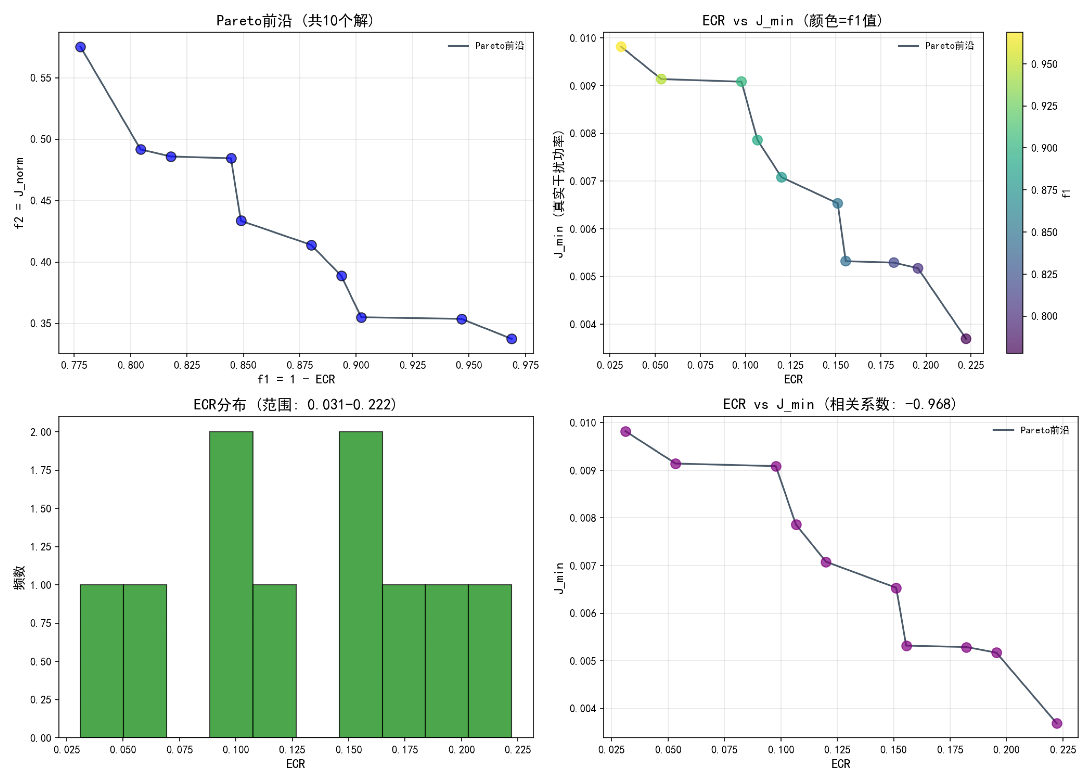
\includegraphics[width=0.86\linewidth]{figures/13_challenging_scene.pdf}
\caption{Challenging场景综合结果。}
\label{fig:challenging_scene}
\end{figure}

\begin{table}[!htbp]
\centering
\small
\caption{Challenging场景结果汇总}
\label{tab:challenging_summary}
\begin{tabular}{lc}
\toprule
指标 & 数值 \\
\midrule
Pareto解数量 & 10 \\
ECR范围 & [0.031, 0.222] \\
$J_{\min}$范围 & [0.0037, 0.0098] \\
拐点ECR & 0.151 \\
ECR-$J_{\min}$相关系数 & --0.968 \\
\bottomrule
\end{tabular}
\end{table}

Paper-Aligned场景在雷达方程模型下得到较高ECR区间的非支配解集。拐点解没有把节点全部推向覆盖最大化，而是在覆盖和$J_{\min}$之间保留了折中。图~\ref{fig:paper_aligned_results}显示，节点布局较分散，弱覆盖区域多出现在远离节点或靠近区域角落的位置。图~\ref{fig:paper_aligned_pareto}中的前沿也说明，继续提高ECR通常会压低$J_{\min}$。

Challenging场景的距离衰减更快，整体ECR明显低于Paper-Aligned场景。即便如此，算法仍生成了多个非支配解。该场景的目标值跨度更大，说明节点位置对覆盖结果更敏感；拐点解的ECR也更低，表明传播衰减强度会直接限制有限节点数量下的覆盖上限。

两类场景的传播模型和覆盖难度不同，但均观察到覆盖率扩展与最薄弱任务点压制强度之间的负相关趋势。表~\ref{tab:correlation_summary}和图~\ref{fig:paper_aligned_correlation}给出跨场景相关性验证。该结果应理解为本文测试场景下的经验性权衡，而非严格数学必然性。

\begin{table}[!htbp]
\centering
\small
\caption{跨场景ECR-$J_{\min}$相关系数汇总}
\label{tab:correlation_summary}
\begin{tabular}{lcc}
\toprule
场景 & 相关系数 $r$ & 样本量 \\
\midrule
Paper-Aligned & --0.923 & 7 \\
Challenging & --0.968 & 10 \\
\bottomrule
\end{tabular}
\end{table}

\begin{figure}[!htbp]
\centering
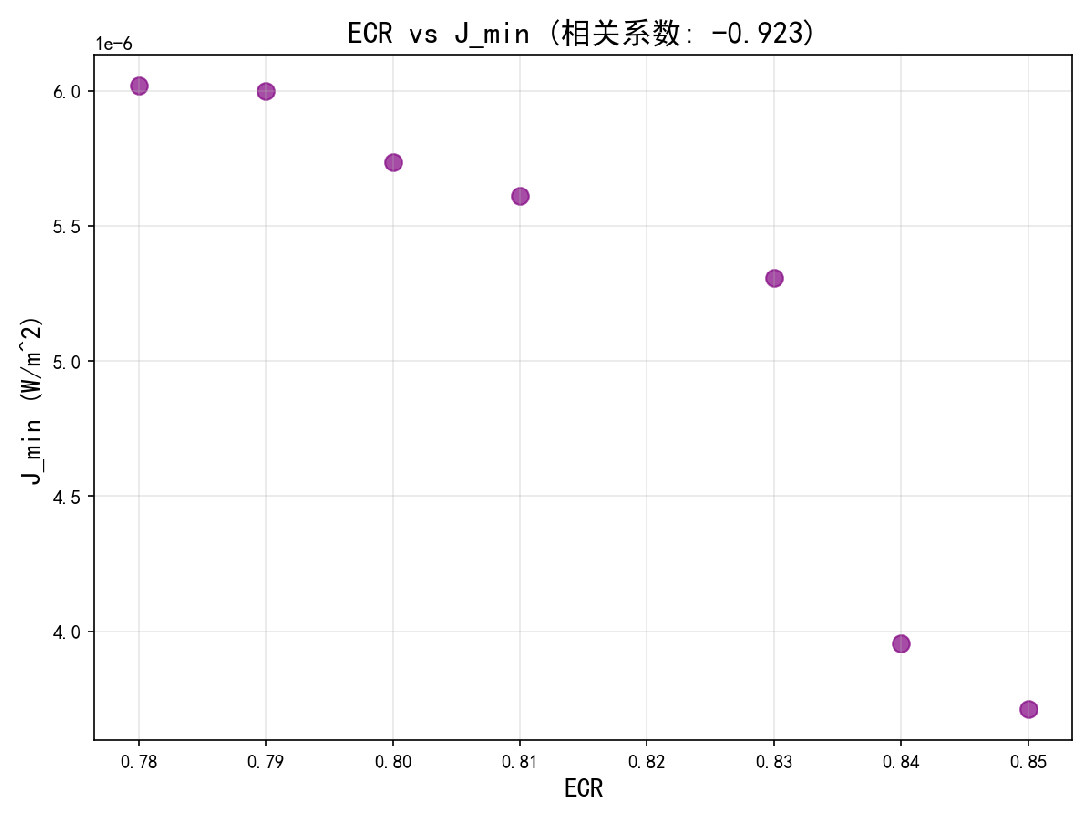
\includegraphics[width=0.82\linewidth]{figures/paper_aligned_correlation.pdf}
\caption{Paper-Aligned场景ECR vs $J_{\min}$相关性分析。}
\label{fig:paper_aligned_correlation}
\end{figure}

相关性结果的负相关来源比较直观：覆盖率目标会把节点往空间上摊开，尽量让更多任务点越过探测阈值；$J_{\min}$目标则会把注意力拉回最弱任务点附近，提高短板位置的到达强度。节点数量固定时，两种需求共享同一组部署资源，所以前沿呈现此消彼长。相关系数只用于说明这种方向性，不替代HV和Spacing等前沿质量指标。

\begin{figure}[!htbp]
\centering
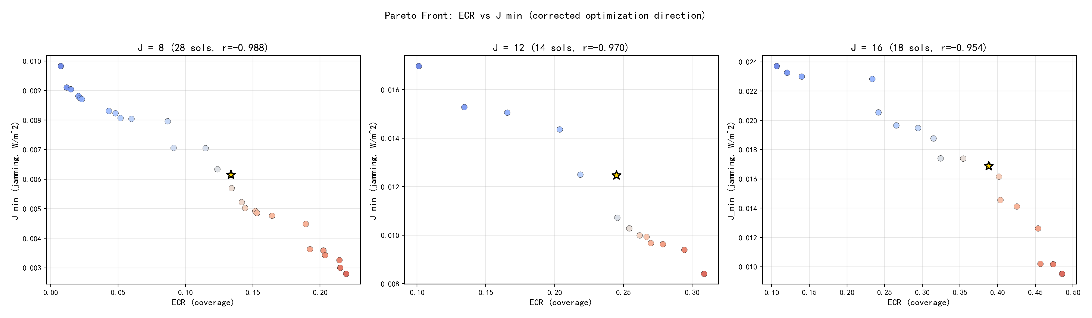
\includegraphics[width=0.86\linewidth]{figures/tradeoff_fixed.pdf}
\caption{不同雷达数量下ECR与$J_{\min}$的权衡。}
\label{fig:tradeoff_fixed}
\end{figure}

任务选择意义体现在图~\ref{fig:tradeoff_fixed}所展示的节点数量变化趋势中。节点更多时，ECR和$J_{\min}$的可达范围整体上移；但在同一节点数量下，解仍沿覆盖率和压制强度的反向方向分布。若任务偏向广域监视，可选ECR较高的方案；若任务偏向重点区域压制，可选$J_{\min}$较高的方案。本文输出的是候选方案集，而不是替使用者固定一个部署点。

表~\ref{tab:baseline_comparison}给出与代表性工作的能力维度比较。该表只做定性说明，不能替代表~\ref{tab:algorithm_comparison}中的同场景定量比较；后者已经显示经典MOEA方法在部分Pareto指标上更强。本文方法的主要特点是把区域约束、空地异构传播、参数调优和公平对比协议放进同一部署流程。

\begin{table}[!htbp]
\centering
\small
\caption{与现有代表性工作的能力对比}
\label{tab:baseline_comparison}
\begin{tabular}{p{0.34\linewidth}cccc}
\toprule
代表性工作 & 边界效应处理 & 异构传播 & 多目标 & 优化效率 \\
\midrule
雷达网络综述~\cite{Javadi2020} & $\times$ & $\times$ & $\times$ & -- \\
NSGA-II雷达部署~\cite{Yan2024} & $\times$ & $\times$ & $\surd$ & 中 \\
非连通区域MSRS部署~\cite{MSRS2024} & $\surd$ & $\times$ & $\times$ & 中 \\
分布式雷达拓扑优化~\cite{Cao2026NSMOPSO} & $\times$ & $\times$ & $\surd$ & 中 \\
MOPSO-DT~\cite{Han2025} & $\surd$ & $\times$ & $\surd$ & 中 \\
本文方法 & $\surd$ & $\surd$ & $\surd$ & 高 \\
\bottomrule
\end{tabular}
\end{table}

综合来看，本章实验分别检查了优化器表现、边界可达性、内部参数和建模假设。当前MOPSO-DT配置没有在所有Pareto质量指标上领先；NSGA-II、MOEA/D和SPEA2在部分指标上仍然更强。本文保留下来的结论是：在复杂区域和空地异构传播同时存在时，所提流程能够把合法位置映射、物理目标计算和非支配方案输出连接起来，结果也能回到具体任务取舍上解释。

因此，本章更强调部署流程的可解释性，而不是把某个优化器包装成普遍最优。后续若加入三维地形、动态任务点或更复杂的电磁传播模型，还需要沿用同一公平评价协议重新验证算法配置和建模假设。

\FloatBarrier

\paragraph{调参结果的解释}
参数调优实验的目的在于观察不同惯性权重、档案选择和变异设置对搜索结果的影响，而不是从单次实验中给出绝对固定的最优参数。实验结果表明，较强的探索能力有助于扩大 Pareto 前沿覆盖范围，但也可能带来间距指标波动；较保守的搜索策略可能获得更稳定的局部结果，却也可能遗漏部分代价较低或性能较高的候选区域。因此，本文在后续实验中采用的参数组合更强调整体流程的稳定性和可解释性，而不是只追求某一个评价指标的单点最优。这样的处理方式与多目标优化问题的特点一致，即算法配置需要在收敛性、多样性和运行代价之间取得平衡。

\paragraph{算法对比结果的解释}
与 NSGA-II、MOEA/D、SPEA2 等经典多目标算法相比，本文方法的特点主要体现在部署问题结构的利用上，而不应简单表述为所有指标全面占优。经典算法在部分指标上可能获得更高的超体积或更好的前沿分布，这与其成熟的种群进化机制有关；本文方法的重点则在于将区域分解、坐标变换和 MOPSO 搜索结合起来，使算法更直接地服务于不规则区域雷达部署问题。换言之，对比实验说明本文方法在给定场景下具有一定竞争力，但其价值不仅来自最终数值排名，还来自模型约束、部署可行性和结果解释之间的一致性。

\paragraph{边界处理实验的解释}
边界分析实验用于观察坐标变换和直接物理空间搜索之间的差异。直接在物理空间中更新位置时，粒子可能频繁越过任务边界，随后再被裁剪或投影回可行域，这可能造成搜索轨迹与原始速度方向不一致，影响边界附近候选解的稳定性。坐标变换方法通过在参数空间内保持连续更新，再映射到真实区域，使边界约束较自然地嵌入候选解生成过程。实验结果中不同方法的 ECR、$J_{\min}$ 和超体积差异，反映出边界处理策略可能对可行解质量和前沿形态产生影响。

\paragraph{数据一致性与结论边界}
本文实验表格和图形均围绕同一组评价目标展开：ECR 表示部署代价，$J_{\min}$ 表示最小观测性能，HV 和 Spacing 用于评价非支配解集。图中展示 Pareto 前沿时采用物理指标坐标，算法内部使用的归一化目标只用于优化计算，不作为最终物理量解释。基于现有实验结果，可以认为本文方法在给定场景下能够生成具有合理权衡关系的部署候选方案，并表明区域分解和坐标变换对边界约束处理具有一定作用。但本文不将结果推广为所有雷达网络部署问题中的绝对最优结论，后续仍需在更多区域形状、雷达参数和任务约束下进一步验证。

\section{本章小结}

本章围绕多算法对比、边界效应、参数调优、消融实验和跨场景权衡给出了验证结果。实验显示，本文配置没有在所有Pareto质量指标上超过经典MOEA方法，但能够在复杂区域约束、空地异构传播和非支配部署方案输出之间形成统一流程；边界实验和相关性分析也说明，覆盖范围与最薄弱点压制强度需要作为任务取舍共同呈现。
